\section{Discussion and Results}
\label{sec:results}

In this section we provide our results from evolving the Adabot.
%
Specifically, we evolved the Adabot in two environments (with and without obstacles) and with two different controllers. Each of these four experiments is repeated 20 times.
%
Finally, we discuss principles that can be learned from these experiments.


\subsection{Fitness Calculations}

% As discussed in the previous section, the goal of our robot is to visit a set of coordinates (way-points) in sequence.
%
Here, Adabot's goal is to visit a set of coordinates (way-points) in sequence.
%
During a single simulation, the device has 30 ($t_\mathit{max}$) seconds to visit \textbf{four} predefined way-points, but the simulation will terminate as soon as the fourth way-point is reached.
%
Fitness is calculated as follows:

%\vspace{-0.15in}

\begin{align}
    f &= 2w + (1-\frac{\min[d, d_\mathit{max}]}{d_\mathit{max}}) + \frac{(t_\mathit{max} - t)}{t_\mathit{max}}
\end{align}

\noindent
where $w$ represents the number of way-points reached, $d$ and $d_\mathit{max}$ denote the distance to the next way-point and a scaling factor for distances, respectively, and $t$ denotes the time transpired.
%
This function is meant to provide a smooth gradient for generating controllers that quickly navigate to all way-points in order.
%
The first part of the equation ensures that the CMA-ES algorithm heavily favors any controller that reaches even a single way-point; values for this component range from 0 to 8.
%
Next, a distance component is added to reward solutions that drive near the next way-point in sequence, but do not reach all four. This is particularly useful at the beginning when solutions are at an early stage of evolution.
%
The distance component results in a value scaled between 0 and 1.
%
Since the simulation ends once all four way-points have been reached, the time component will be a value between 0 (zero time remaining) and 1 (all four way-points are reached in an instant).
%
The time component is meant to favor any controllers that solve the task quickly.
%
Thus, the maximum possible fitness is 10.


\subsection{Evolution Without Obstacles}

In our first experiment, \emph{FSM-0-1}, we evolve the fifteen parameters found in Tables~\ref{tbl:params-physical} (physical) and~\ref{tbl:params-fsm} (control) in an environment without obstacles.
%
The naming scheme for our experiments indicates the controller type (\emph{FSM} or \emph{ANN}), the maximum number of potential obstacles (0 or 40), and the number of trials per fitness evaluation (1 or 2).
%
Plots of fitness vs iteration are shown in \figref{fig:fitness-vs-iteration} (this figure shows the fitness values for all four experiments).
%
In this first experiment, there are zero obstacles and therefore the environment will always be the same. In later experiments, each fitness evaluation includes two trials with randomly generated obstacles.
%
As shown in the figure, in all replicate experiments the Adabot reaches all four way-points in approximately 10 seconds, which corresponds to a fitness value of 9.7.
%
The population quickly converges on a final value, likely because this experiment was seeded with a hand-designed set of parameters known to achieve good results (see Table~\ref{tbl:params-fsm}); the evolved results, however, quickly outperform the hand-chosen values.
%
This experiment serves as a convenient baseline with which the others can be compared.

\begin{figure}[!ht]
    \centering

    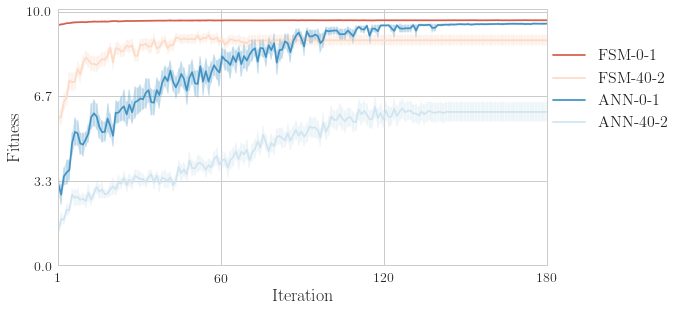
\includegraphics[width=\columnwidth]{figures/4-results/fitness.png}

    %\vspace{-0.1in}

    \caption{Plots for the maximum fitness found in each of the four experiments. Shaded regions indicate confidence intervals of one standard deviation from the mean for the 20 replicates of each experiment. The maximum possible fitness is 10, and fitness values above 2 indicate that Adabot was able to reach at least one way-point.}
    \label{fig:fitness-vs-iteration}

    %\vspace{-0.1in}
\end{figure}


The second experiment, denoted \emph{ANN-0-1}. also reaches a fitness value of 9.7, which shows that the an ANN can effectively perform the task of navigating the robot to a sequence of points.
%
For this experiment, 17 total parameters were evolved: the four physical characteristics listed in \tblref{tbl:params-physical} and the 13 ANN parameters discussed in the previous section.
%
Although both of these experiments reach the same final fitness value, an examination of \figref{fig:fitness-vs-iteration} shows that the ANN result takes longer to evolve--roughly 120 iterations compared with less than 10 iterations for the FSM.
%
This can be explained by the lack of a seed controller and the fact that, unlike an FSM, an ANN must learn the entire solution from scratch.


\figref{fig:0-1-best-trajectories} depicts the trajectories taken by the best performing controllers from these two experiments.
%
Although these trajectories look similar, there is one key difference: the ANN actively controls only one wheel. FSMs, on the other hand, rotate both directions in-place, which is why there are sharper turns in the left plot.


\begin{figure}[!ht]
    \centering

    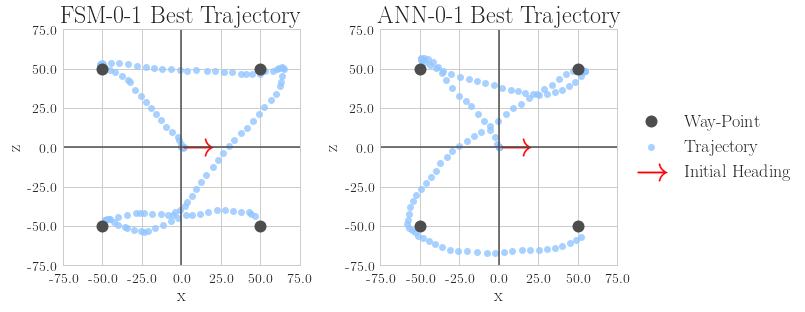
\includegraphics[width=\columnwidth]{figures/4-results/0-1-best_trajectories.png}

    %\vspace{-0.12in}

    \caption{Trajectories of the best evolved individual for the first two experiments: FSM-0-1 and ANN-0-1. No obstacles were present for these trajectories.}
    \label{fig:0-1-best-trajectories}

    %\vspace{-0.1in}
\end{figure}


% This tactic can be more easily seen in \figref{fig:ANN-0-1-best-speed}.
\figref{fig:ANN-0-1-best-speed} shows the wheel speeds for the best FSM and ANN controllers.
%
% This figure shows that t
The evolved ANN perpetually sets the right wheel to its maximum speed.
%
The ANN moves forward by setting its left wheel to the same value, and turns by making the left wheel rotate in the opposite direction.
%
Effectively, the ANN can only turn left, however, this is not a problem for the relatively simple task at hand.



\begin{figure}[!ht]
    \centering

    \subfloat[]{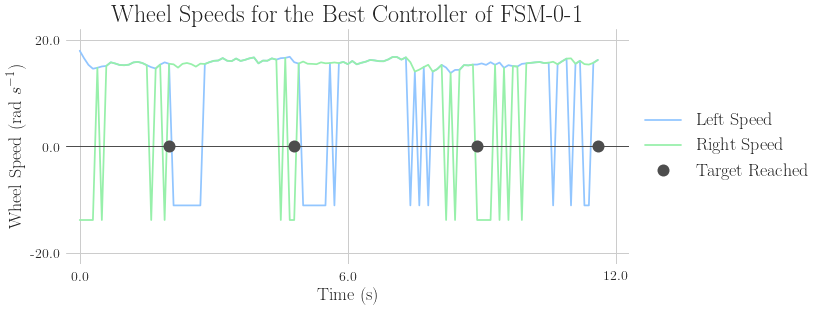
\includegraphics[width=\columnwidth]{figures/4-results/FSM-0-1-best_speed.png}}

    %\vspace{-0.08in}

    \subfloat[]{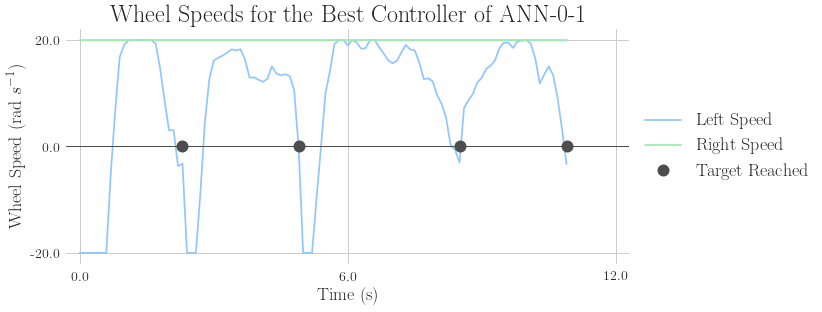
\includegraphics[width=\columnwidth]{figures/4-results/ANN-0-1-best_speed.png}}

    %\vspace{-0.08in}

    \caption{Left and right wheel speeds for the best evolved solutions for \emph{FSM-0-1} (a) and \emph{ANN-0-1} (b).}
    \label{fig:ANN-0-1-best-speed}

    %\vspace{-0.1in}
\end{figure}


\figref{fig:0-1-best-params} provides a comparison of the fitness values and evolved physical characteristics for these two experiments.
%
This figure only shows results for the combined final populations of all replicate experiments.
%
From this figure, we can establish what will be good physical characteristics for the Adabot when it does not face any obstacles.
%
Specifically, \emph{WheelBase} and \emph{TrackWidth} should be 8.5~\si{cm} and 11.5~\si{cm}, respectively, \emph{WheelRadius} should be 3~\si{cm}, and \emph{StrutCount} does not matter since the struts are not extended.


\begin{figure}[!ht]
    \centering

    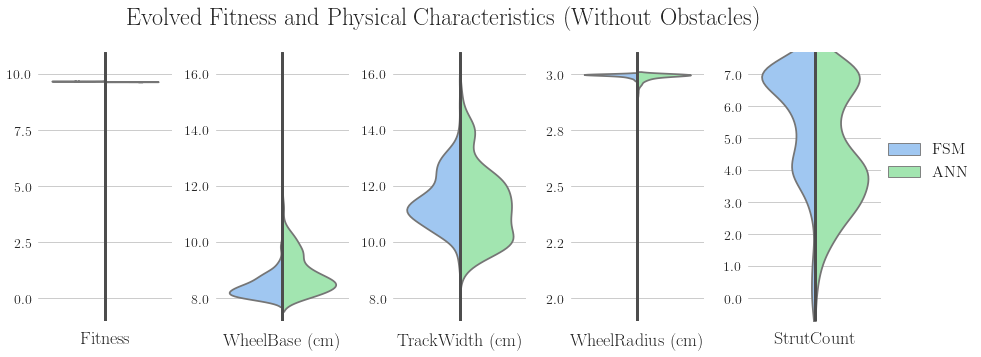
\includegraphics[width=\columnwidth]{figures/4-results/0-1-best_params.png}

    %\vspace{-0.1in}

    \caption{Distributions for the evolved fitness values and physical characteristics for the combined final populations of the \emph{FSM-0-1} (left side) and \emph{ANN-0-1} (right side) experiments. The y-axis limits are the parameter limits allowed during evolution.}
    \label{fig:0-1-best-params}

    %\vspace{-0.1in}

\end{figure}


Finally, \figref{fig:FSM-best-params} plots the distributions for all evolved FSM parameters.
%
It is worth noting that in the absence of obstacles, neither the evolved FSMs or ANNs extend the struts.
%
This result is not unexpected as any extension would result in a reduced speed (due to the scaling mentioned previously), and the struts are not needed when obstacles are not present.
%
Also of interest is the evolved symmetry of the FSM.
%
Specifically, the threshold values and speeds evolved for the \emph{Left} and \emph{Right} states are nearly perfect mirror images of each other.


\begin{figure*}[!ht]
    \centering

    % \subfloat[]{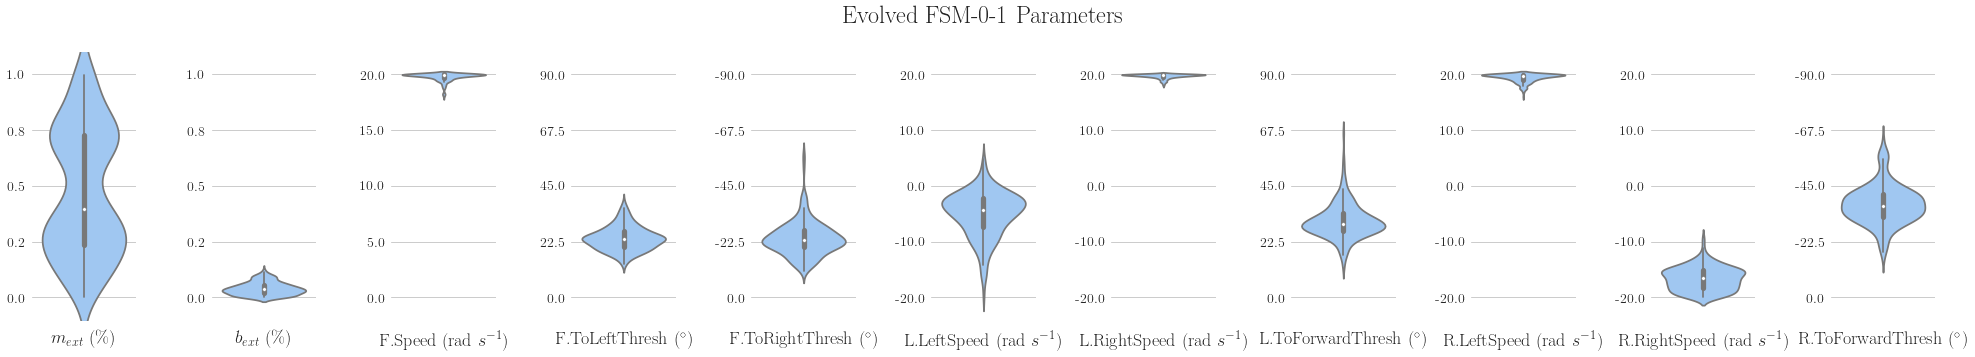
\includegraphics[width=\textwidth]{figures/4-results/FSM-0-1-best_params.png}}
    % \hfil
    % \subfloat[]{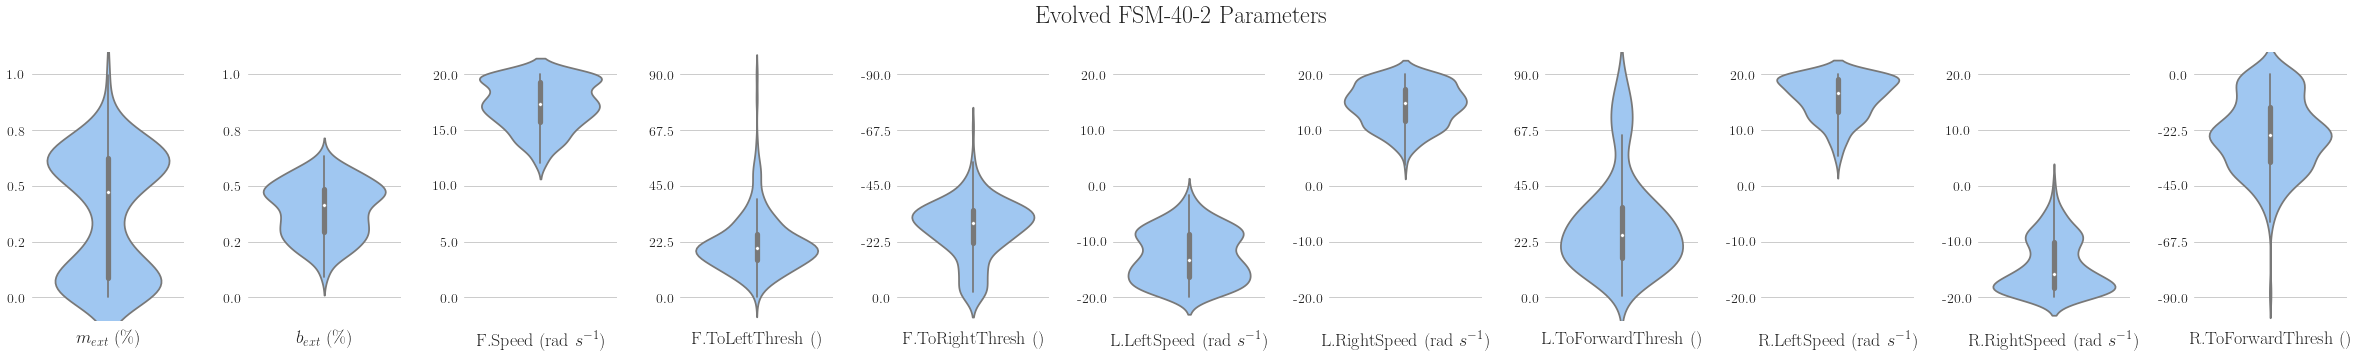
\includegraphics[width=\textwidth]{figures/4-results/FSM-40-2-best_params.png}}

    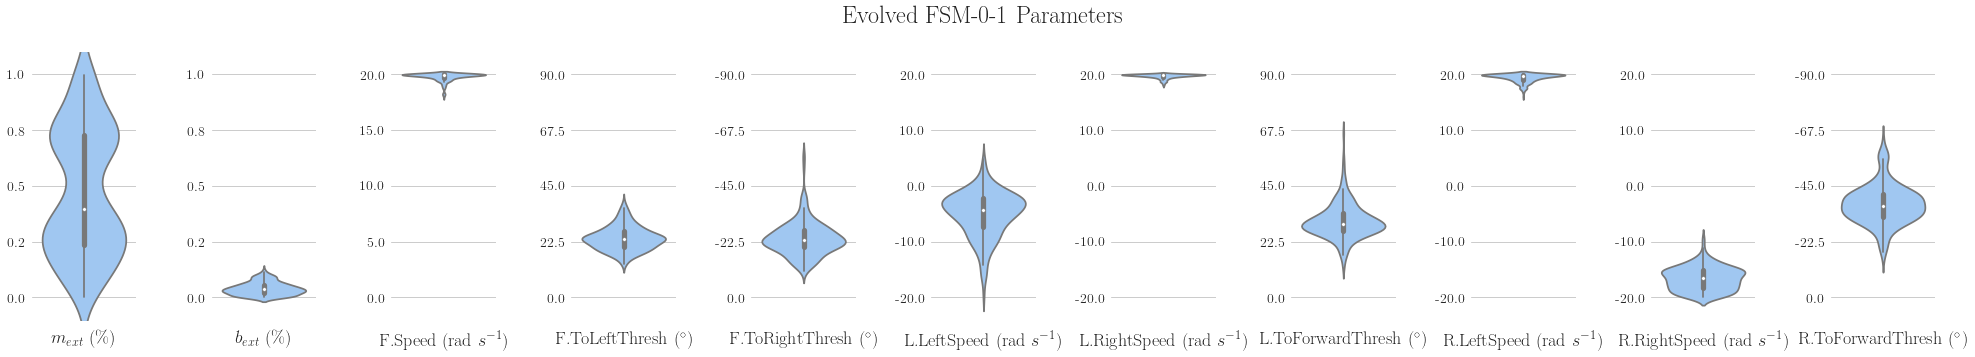
\includegraphics[width=\textwidth]{figures/4-results/FSM-0-1-best_params.png}

    %\vspace{-0.08in}

    % \caption{Distributions for all evolved FSM parameters for the \emph{FSM-0-1} and \emph{FSM-40-2} experiments.}
    \caption{Distributions for all evolved FSM parameters for the \emph{FSM-0-1} experiment. These parameters are described in Figure~\ref{fig:fsm}(a) and Table~\ref{tbl:params-fsm}.}
    \label{fig:FSM-best-params}
\end{figure*}


\subsection{Evolution With Obstacles}

% Best BNN
% '30 40 0 0.08218 0.1193 0.02994 5 0 3.983 3.718 -0.6273 -3.185 -0.1238 -0.6903 1.984 3.977 2.171 2.209 3.999 -0.2371'

% Best FSM
% '30 40 0 0.09734 0.1259 0.02998 6 0.4915 0.3365 0.8207 0.8632 -0.377 -0.7851 0.9327 0.7227 0.6914 -0.9314 -0.6232'

The final two evolutionary experiments are referred to as \emph{FSM-40-2} and \emph{ANN-40-2}.
%
These experiments differ from the previous two in two respects. First, each fitness value is calculated as the average of two trials (where each trial lasts at most 30 seconds), and second, each fitness trial occurs in an environment with around 31 randomly generated obstacles.
%
Utilizing multiple trials during fitness evaluations improves the robustness of the evolved results~\citep{Ruud.SSCI.EvoLearn.2016}.
%
The fitness plots for these experiments appear in \figref{fig:fitness-vs-iteration}.
%
Of note is that the ANNs evolved with obstacles have a greatly reduced maximum fitness. A few individuals achieve a fitness above 9, however, we found that this was only when the randomly generated environment did not pose much difficulty.
%
Videos (and interactive animations) for high fitness individuals can be found here: \emph{FSM-40-2}: \url{https://youtu.be/VXnrwwpE598} (\url{https://goo.gl/NtoVYe}); and \emph{ANN-40-2}: \url{https://youtu.be/q8PFqQps5e4} (\url{https://goo.gl/2xjh6X}).
%
% We have provided videos for the highest fitness individuals from both experiments: \emph{FSM-40-2} example behavior: \url{https://youtu.be/VXnrwwpE598}; and \emph{ANN-40-2} example behavior: \url{https://youtu.be/q8PFqQps5e4}.


% After reviewing the distributions in Figures~\ref{fig:0-1-best-params} and~\ref{fig:40-2-best-params}
Similar to \figref{fig:0-1-best-params}, \figref{fig:40-2-best-params} shows the distributions for the evolved physical characteristics.
%
These distributions have a larger spread due to the randomly generated environments.
%
The values found in these distributions indicate that the presence of obstacles does not have a drastic affect on the evolution of physical characteristics.
%
At first this was unexpected, however, analyzing these values (and visualizing their resulting behaviors) reveals a few basic principles:
(1) for a skid steer robot it is important for the \emph{WheelBase} to be less than the \emph{TrackWidth} (this will reduce the amount of \emph{skidding} and improve controllability),
(2) to maximize velocity \emph{WheelRadius} should be maximized (since we are evolving wheel angular rate a larger wheel will result in a higher velocity), and
(3) as long as the number of struts is greater than 4 the system will be able to navigate the generated environments.
%
The first and second principles match results that we have seen on the physical prototype, and we intend to investigate the third principle in the near future.
%
% This leaves us with control being the most important factor in navigating obstacles.


\begin{figure}[!ht]
    \centering

    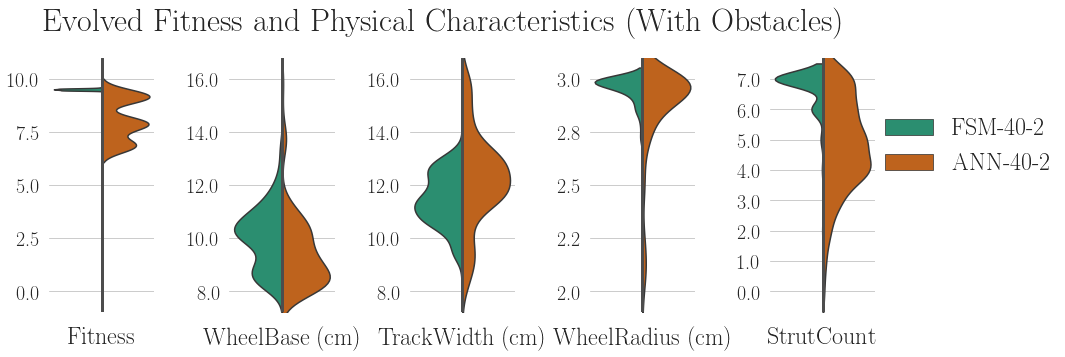
\includegraphics[width=\columnwidth]{figures/4-results/40-2-best_params.png}

    %\vspace{-0.07in}

    \caption{Distributions for the evolved fitness values and physical characteristics for the combined final populations of the \emph{FSM-40-2} (left side) and \emph{ANN-40-2} (right side) experiments. The y-axis limits are the parameter limits allowed during evolution.}
    \label{fig:40-2-best-params}

    % %\vspace{-0.2in}

\end{figure}



While the physical characteristics are similar between the two sets of experiments, control strategies have been adjusted to handle the obstacles.
%
\figref{fig:40-2-best-speed} shows the control patterns for two solutions randomly selected from the best performing individuals of the \emph{FSM-40-2} and \emph{ANN-40-2} experiments.
%
Note that since environments are randomly generated, even though the evolved ANN does not reach all four way-points for this test, it does not mean that it did not do so during fitness evaluation.
%
The most important feature of the plots in \figref{fig:40-2-best-speed} are that the evolved controllers are operating at reduced speeds.
%
% Examining the evolved values in \figref{fig:FSM-best-params} shows that for at least the \emph{FSM-40-2}, the evolved speeds are still near the maximum allowed value.
%
Examining the evolved FSM values, we see that nearly identical values are discovered for all parameters except $b_{\mathit{ext}}$
(a set of distributions similar to \figref{fig:FSM-best-params} has been omitted to save space).
%
In the experiment with no obstacles, $b_{\mathit{ext}}$ converged to zero, however, for this experiment $b_{\mathit{ext}}$ converged to 0.45.
%
A higher value for $b_{\mathit{ext}}$ results in the struts always being extended (even when no obstacle has been encountered).
%
Thus, these behaviors are slower because the struts are required to climb obstacles.

% the cause of the slower behavior is that the controllers are using the struts to improve mobility in the face of obstacles.
%
% This can also be seen by looking at the evolved values for $b_{\mathit{ext}}$, without obstacles this value is near zero, and with obstacles this value is closer to 0.45.




\begin{figure}[!ht]
    \centering

    \subfloat[]{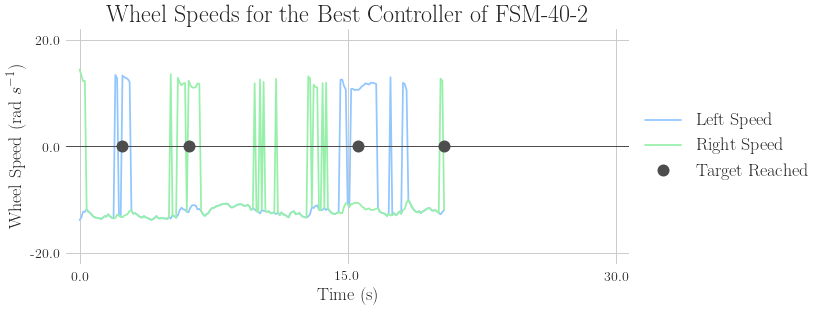
\includegraphics[width=\columnwidth]{figures/4-results/FSM-40-2-best_speed.png}}

    %\vspace{-0.08in}

    \subfloat[]{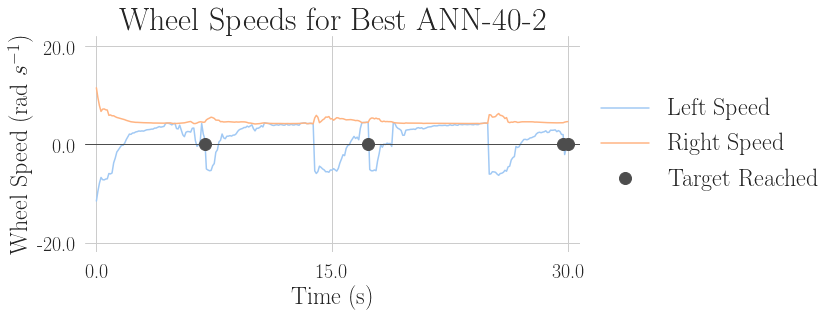
\includegraphics[width=\columnwidth]{figures/4-results/ANN-40-2-best_speed.png}}

    %\vspace{-0.08in}

    \caption{Left and right wheel speeds for the best evolved FSM (a) and ANN (b) in a randomly generated environment that includes obstacles.}
    \label{fig:40-2-best-speed}

    %\vspace{-0.2in}

\end{figure}





% The final set of evolved parameters to examine is those of the neural network.
%
Directly examining the evolved weights of a neural network provides only a limited view of the resulting behavior. Likewise, comparing each input's effect on each output in isolation obscures the resulting behaviors.
%
For example, some output values are only active when some combination of multiple input values are provided.
%
Thus, in \figref{fig:ANN-40-2-best-ann-map} we provide all pairwise input relationships on the output for the speed of the left wheels in the form of heat-maps.
%
These heat-maps were generated using a parameter sweep over all possible input combinations. Each square represents the output value given the two input values on the x- and y-axes averaged over all possible values for the remaining input.
%
% Looking at the second and third rows in this figure we can see that for any combination of input values the right wheel is always rotating at a constant forward speed and the struts are always fully extended, respectively.
%
As was the case for the \emph{ANN-0-1} experiment, all navigation is handled by driving the left wheel at different speeds, and so we have not provided heat-maps for the wheel strut and right speed outputs.
%
Examining the figure shows that the left wheel's speed has a positive linear relationship with both $\omega_e$ and $\alpha_{\mathit{target}}$, and that $\alpha_{\mathit{target}}$ has the greatest effect on control (since it is used to turn the robot towards the target).
%
% As any of the inputs are increased, so to does the left wheel speed.


In both experiments including obstacles, the evolved controllers extended the struts and never fully retracted them.
%
However, there is a clear advantage to retracting the struts: the robot has a higher maximum allowed speed.
%
Thus, it is likely an issue with using the differential drive model to calculate the error.
%
We have identified two sources of error with the simple model: (1) it does not take into account that when the struts are extended the wheel has a larger effective radius, and (2) the model does not take into account the noisy nature of a skid steering and extended struts.


\begin{figure}[!ht]
    \centering

    %\vspace{-0.05in}

    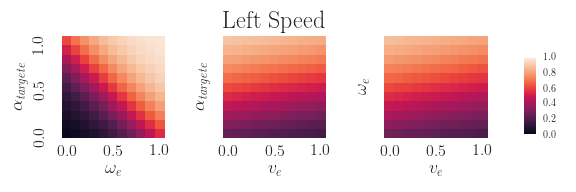
\includegraphics[width=\columnwidth]{figures/4-results/ann_map.png}

    %\vspace{-0.1in}

    \caption{Heat-maps showing the relationship between input and output for the left wheels of the best evolved ANN. A light shade indicates that the wheel is at its maximum forward rate, and a dark color indicates that it is at its maximal reverse rate. All input and output values are scaled between 0 and 1. Outputs area only shown for the left wheel has it was the only ANN output that exhibited a variety of different values.}
    \label{fig:ANN-40-2-best-ann-map}

    % %\vspace{-0.08in}

\end{figure}


In summary, regarding the optimization of the Adabot system we found that:

\begin{enumerate}

\item Similar physical characteristics are optimal with and without obstacles in the environment.

\item The speed of the left and right wheels should have a linear relationship with $\alpha_{\mathit{target}}$ (rather than a discrete relationship as is the case with the current FSM).

\item The task can be solved by controlling only a single wheel, though, this is likely not a desirable trait. In future work, we plan to add an evolutionary pressure so that the evolved ANNs turn in both directions.

\item Controlling the strut will require a more complex model of the robots dynamics. Once the struts are extended, it is difficult to discern when they should be retracted.

\end{enumerate}

Taking these observations into account, we developed a hybrid two-state controller. The controller is in \emph{Left} when $\alpha_{\mathit{target}}$ is greater than zero and in \emph{Right} otherwise. Equations for these states are as follows:

% %\vspace{-0.1in}

\begin{align}
    \alpha_\mathit{scale} &= 2\cdot(1 - \frac{\alpha_{\mathit{target}}}{\pi}) - 1\\
    \mathit{Left}_\mathit{left} &= -\mathit{MAXRAD} \cdot \alpha_\mathit{scale}\\
    \mathit{Left}_\mathit{right} &= \mathit{MAXRAD}\\
    \mathit{Right}_\mathit{left} &= \mathit{MAXRAD}\\
    \mathit{Right}_\mathit{right} &= \mathit{MAXRAD}\cdot \alpha_\mathit{scale}
\end{align}

\noindent
where $\alpha_\mathit{scale}$ is $\alpha_{\mathit{target}}$ scaled between -1 and 1. This simple hybrid controller is able to visit all way-points in 9.9 seconds, which is one tenth of a second faster than the evolved controllers reported above. The controller also works well in the presence of obstacles when the struts are extended 10\%. Overall, this hybrid controller provides a smoother motion and good performance. For future work, we intend to evolve this hybrid controller along with a more sophisticated approach to handling strut extension.
